\documentclass[12pt]{article}
\usepackage[margin=1in]{geometry}
\usepackage{graphicx}
\usepackage{amsmath}
\usepackage{hyperref}
\usepackage{appendix}
\usepackage{color}

\newcommand{\fixme}[1]{\textcolor{darkred}{\bf FIXME: #1}}
\newcommand{\s}[1]{{\mbox{\scriptsize #1}}}

\begin{document}

\section{Introduction}

The muon endcap was aligned using information from four different
sources: photogrammetry, the Muon Endcap Alignment System, tracks from
beam-halo muons, and tracks from collisions muons.  Some of these
sources of information are orthogonal, while others provide for
cross-checks between the different systems.  To combine information,
alignment corrections were applied in a well-defined sequence, such
that each step benefits from the previous.  Potentially interdependent
corrections were iterated to obtain a mutually consistent solution.

Below are the sources of alignment information and the order of their
application.  Global CMS coordinates are defined in [ref]; local
coordinates are defined with respect to the CSC chambers, with $x$
pointing approximately in the global $r\phi$ direction, $y$ in the
radial direction away from the beamline, and $z$ collinear with CMS
global $z$.  Rotation angles $\phi_x$, $\phi_y$, and $\phi_z$ are
rotations around the corresponding local axes.  (See
Fig.~\ref{fig:csc_coordinates} for a diagram of relevant coordinates.)

\begin{figure}
\begin{center}
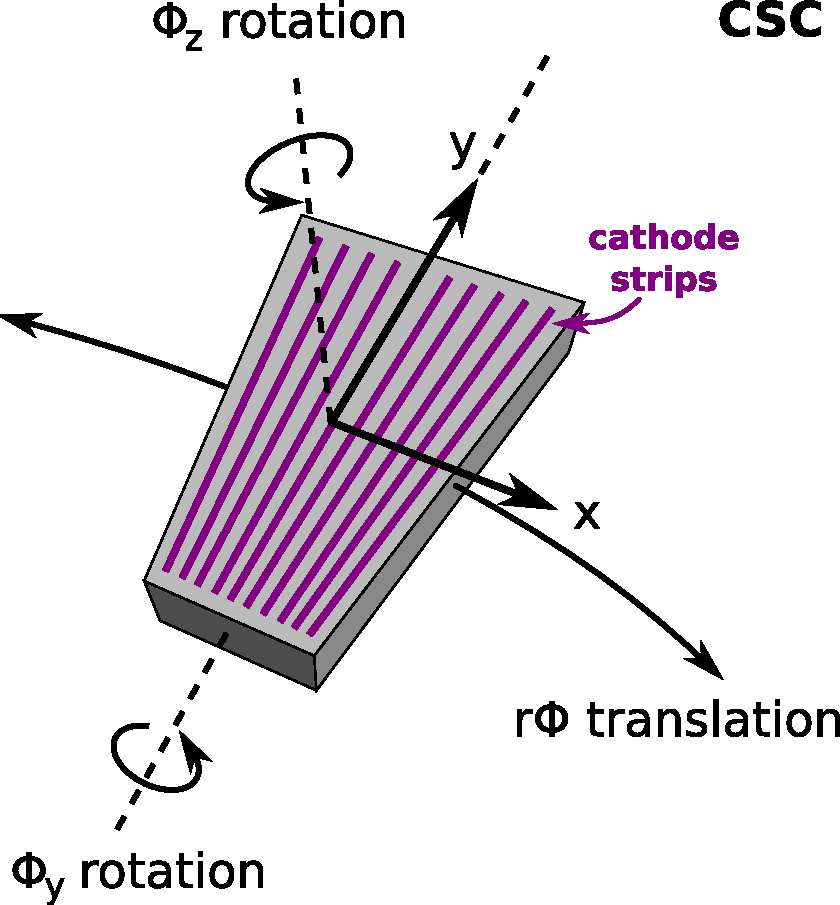
\includegraphics[width=0.3\linewidth]{csc_coordinates.pdf}

\caption{Schematic CSC chamber, indicating the local coordinate
  system. \label{fig:csc_coordinates}}
\end{center}

\end{figure}

\begin{enumerate}
\item Photogrammetry [ref]: alignment derived from a set of
  photographs taken in 2007, establishing local coordinates $x$, $y$,
  $z$, $\phi_x$, and $\phi_z$ for chambers relative to the disks on
  which they are mounted.  Two points were measured on each chamber,
  and these points are on the local $y$ axis (hence the $\phi_y$
  degree of freedom is unavailable).  The disks have subsequently been
  moved, with all chambers attached.
\item Muon Endcap Alignment System [ref]: a system of three lasers
  crossing the face of each disk, six lasers parallel with the
  beamline crossing all disks, and calipers measuring the $z$ spacing
  between disks.  This system is highly sensitive to the large
  displacements and bowing of disks in the CMS magnetic field, and
  therefore supplied corrections to the photogrammetry measurement
  from the zero-field state to the full-field state in local $\phi_x$
  and $z$.
\item Entrance angles of tracks from the tracker: systematic
  discrepancies between the entrance angles predicted by muons from
  the tracker and entrance angles measured by the muon chambers
  themselves were used to determine $\phi_y$.
\item Chamber alignment with beam-halo muons [ref]: relative local $x$
  and $\phi_z$ of chambers derived from beam-halo tracks passing
  through pairs of adjacent chambers.  Since the tracks are propagated
  short distances through low density material, propagation errors are
  minimal, but since the measurements have no external reference, the
  results are only valid for relative positions of chambers within
  each CSC ring.
\item Ring alignment with collisions muons: global $x$, $y$, and
  $\phi_z$ corrections for pre-aligned rings relative to the CMS
  tracker.  Tracks were propagated through material and inhomogeneous
  magnetic fields, but the alignment was simplified by the assumption
  that each ring is internally well-aligned.
\end{enumerate}
The geometry produced after step \#5 was cross-checked using beam-halo
muons propagated through the whole endcap (sensitive to a different
set of systematic uncertainties), and steps \#4 and \#5 were iterated
for mutual consistency.

\section{Measurement of disk bending with the Muon Endcap Alignment System}

\section{Alignment of $\phi_y$ angles}

Several attempts were made to align the $\phi_y$ angles of chambers,
but method with the most precision and fewest assumptions uses tracks
propagated from the tracker.  All track parameters are determined by
the tracker, and the full CMS propagation model is used to estimate
how a muon with a given trajectory will navigate through the material
and magnetic field to the CSC chambers.  In each chamber, the
propagated $dx/dz$ entrance angle of the track is compared with the
entrance angle measured by the chamber, and systematic differences are
interpreted as a misalignment of the chamber
(Fig.~\ref{fig:phiy_alignment}).  Entrance angles are less sensitive
to potential propagation errors than positions, and the interpretation
of discrepancies as chamber misalignments was verified in extreme
cases by the fact that track-chamber differences (``residuals'')
are sharply discontinuous at the boundaries between chambers.

\begin{figure}
\begin{center}
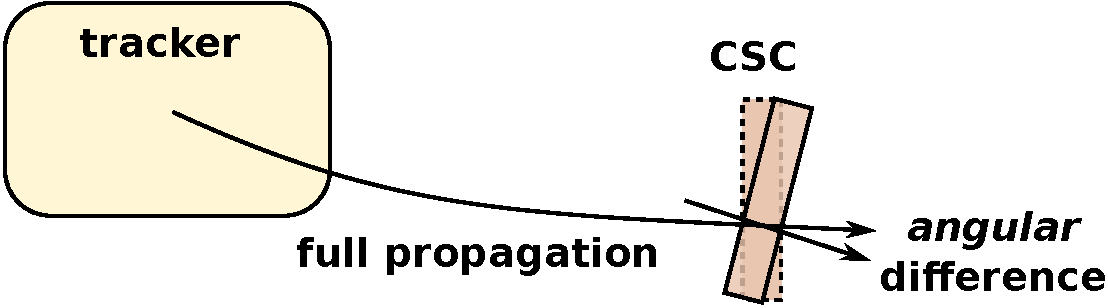
\includegraphics[width=0.5\linewidth]{phiy_alignment.pdf}
\end{center}

\caption{Schematic of CSC $\phi_y$ alignment using tracks from the tracker. \label{fig:phiy_alignment}}
\end{figure}

Figure~\ref{fig:mem3phiy_all} presents corrections in one ring
(ME$-$3/1) compared with measurements of the same parameter using
other techniques.  The $\phi_y$ angles of chambers in all rings were
measured using the tracker-propagation technique, while other methods
were limited to different subsets of rings (ME$-$3/1 is the only ring
in which all could be compared).  From the raw residuals represented
as a color scale in the plot, we can see discontinuities along the
borders between chambers, demonstrating that the systematic
differences are related to the chambers, rather than errors in track
propagation.  (It would be highly unlikely for propagations errors
unrelated to the chambers to deviate exactly at the boundaries of the
chambers.)  The ``LHC pointing'' method assumes that beam-halo muons
observed in zero magnetic field point back to a straight, infinitely
long beamline.  The ``BH overlaps'' (beam-halo overlaps) methods use
beam-halo tracks passing through pairs of neighboring CSCs, much like
the method described in the next section, but applied to $\phi_y$
rather than $x$ and $\phi_z$.  Taken together, these measurements
represent two years of $\phi_y$ monitoring, yet they agree well at
the level of 1--2~mrad.

\begin{figure}
\begin{center}
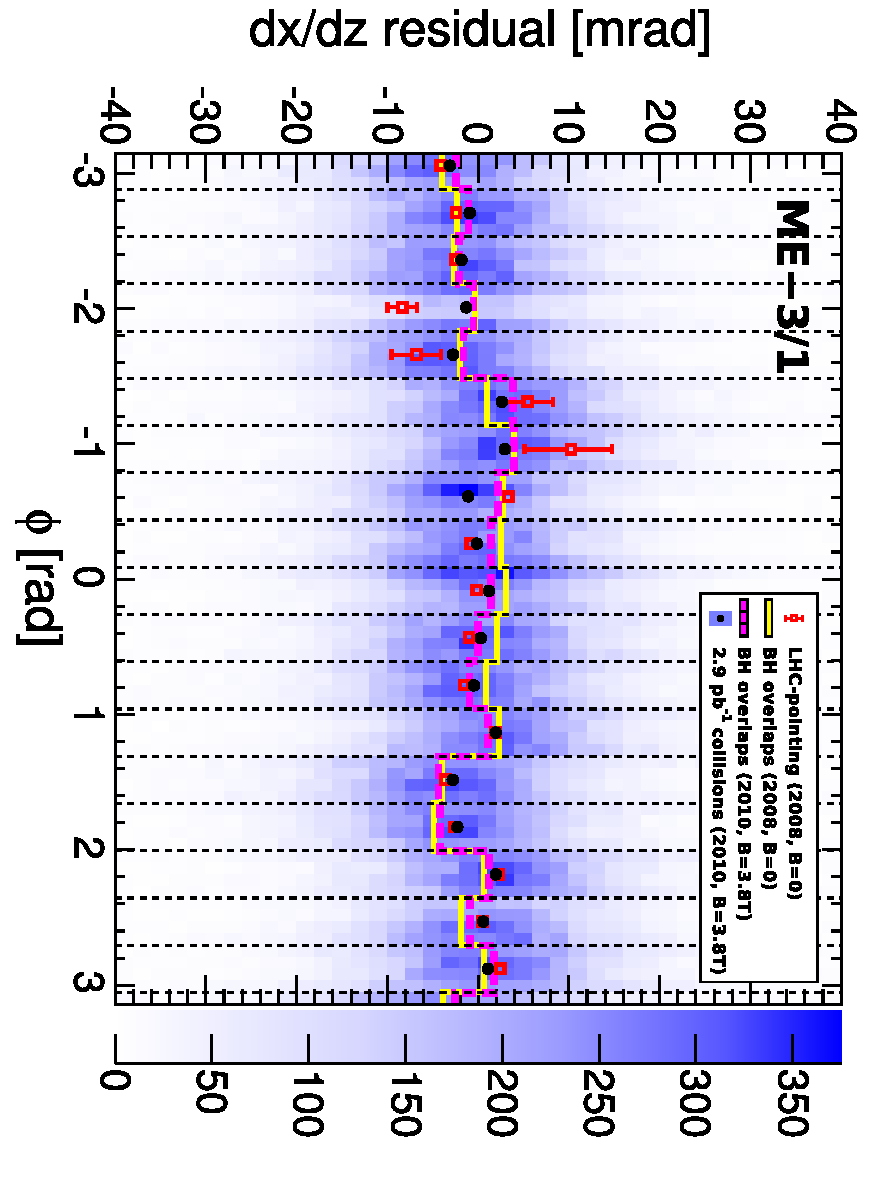
\includegraphics[height=0.6\linewidth, angle=90]{mem3phiy_all.pdf}
\end{center}

\caption{Comparison of $\phi_y$ measurements using several different
  methods: zero-field beam-halo trajectories from the LHC beamline
  (red open squares), zero- and full-field measurements using tracks
  crossing the edges of CSCs (histograms), and entrance angle
  residuals from the tracker (black points and color-scale
  background).  The color-scale represents the distribution of all
  residuals versus $\phi$, while the black points are average
  residuals per chamber. \label{fig:mem3phiy_all}}
\end{figure}

\section{Internal-ring alignment using beam-halo tracks}

CSC chambers overlap slightly along their edges, and muons passing
through these narrow regions provide information about the relative
displacement of the neighboring chambers.  Because of the short
distances between the chambers and the lack of heavy material between
them, straight-line propagations of the muon trajectory are precise at
the level of 1.4~mm RMS (compared to tens of mm for tracks propagated
from the tracker, depending on momentum).  A systematic offset in the
difference between track-segments propagated from each chamber to a
plane equidistant between them (the ``overlap residual'') is
interpreted as a relative displacement between the two chambers
(Fig.~\ref{fig:overlaps}).

\begin{figure}
\begin{center}
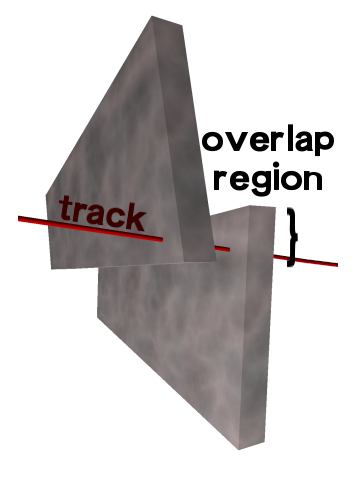
\includegraphics[height=4.5 cm]{overlaps.png} \hspace{1.5 cm}
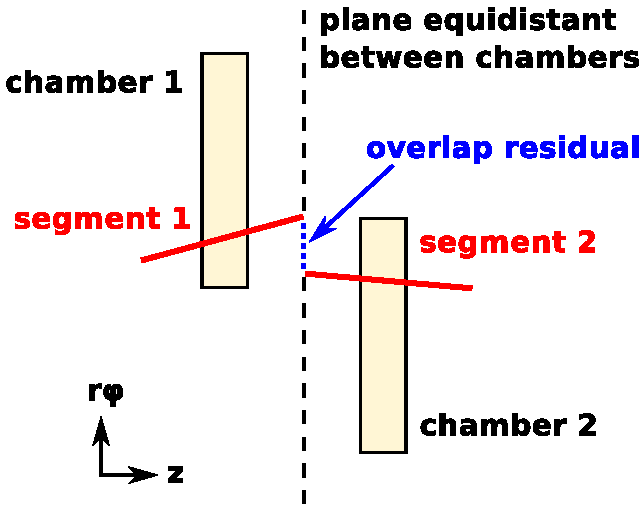
\includegraphics[height=4.5 cm]{overlaps_diagram.pdf}
\end{center}

\caption{Relative alignment information from a muon passing through
  the overlap between two neighboring chambers. \label{fig:overlaps}}
\end{figure}

To produce a complete geometry from the pairwise chamber information,
the following objective function is minimized:
\begin{equation}
\chi^2 = \sum_{m_{ij}}^\s{constraints} \frac{(m_{ij} - A_i +
  A_j)^2}{{\sigma_{ij}}^2} + \lambda \left(\frac{1}{N_\s{chambers}} \sum_i^\s{chambers}A_i\right)^2
\label{eqn:minimizeme}
\end{equation}
where $A_i$ are the chamber coordinates to optimize, $m_{ij} \pm
\sigma_{ij}$ are the pairwise chamber measurements, and $\lambda$ is a
Lagrange multiplier to compensate for the fact that the system has no
external reference to define a coordinate system.  Two chamber
coordinates can be measured with high precision using this technique,
$r\phi$ (from an average offset in overlaps residuals) and $\phi_z$
(from a trend in overlaps residuals as a function of local $y$).
Other coordinates are better measured with other methods.  Only one
coordinate is aligned at a time, alternating between $r\phi$ and
$\phi_z$.

Relative alignment information can only be propagated through a
complete graph of alignment constraints, and since there are no
overlaps between chambers in different rings, misalignments between
rings are not corrected with this method.  In addition, some rings are
not fully connected due to one or two dead chambers or dead CFEBs,
affecting the region of overlap.  In these rings, photogrammetry
information is used to fill the gaps, with photogrammetry measurements
introduced as constraints in Eqn.~\ref{eqn:minimizeme}.  Rings
ME$\pm$1/1 have two missing chambers each, but no photogrammetry
measurements to use as constraints.  In this case, we measured the
positions of the chambers neighboring the gaps with tracks from the
tracker and applied them as constraints in the same way.

Figure~\ref{fig:aligned_minus_pg} presents the results of this
alignment by comparing post-alignment chamber positions to
pre-alignment values from photogrammetry.  Although photogrammetry
information was used in the alignment, much larger weights were given
to the beam-halo data.  The level of agreement between the track-based
technique and photogrammetry (0.3--0.6~mm) is smaller than the typical
chamber corrections (2--3~mm).

\begin{figure}
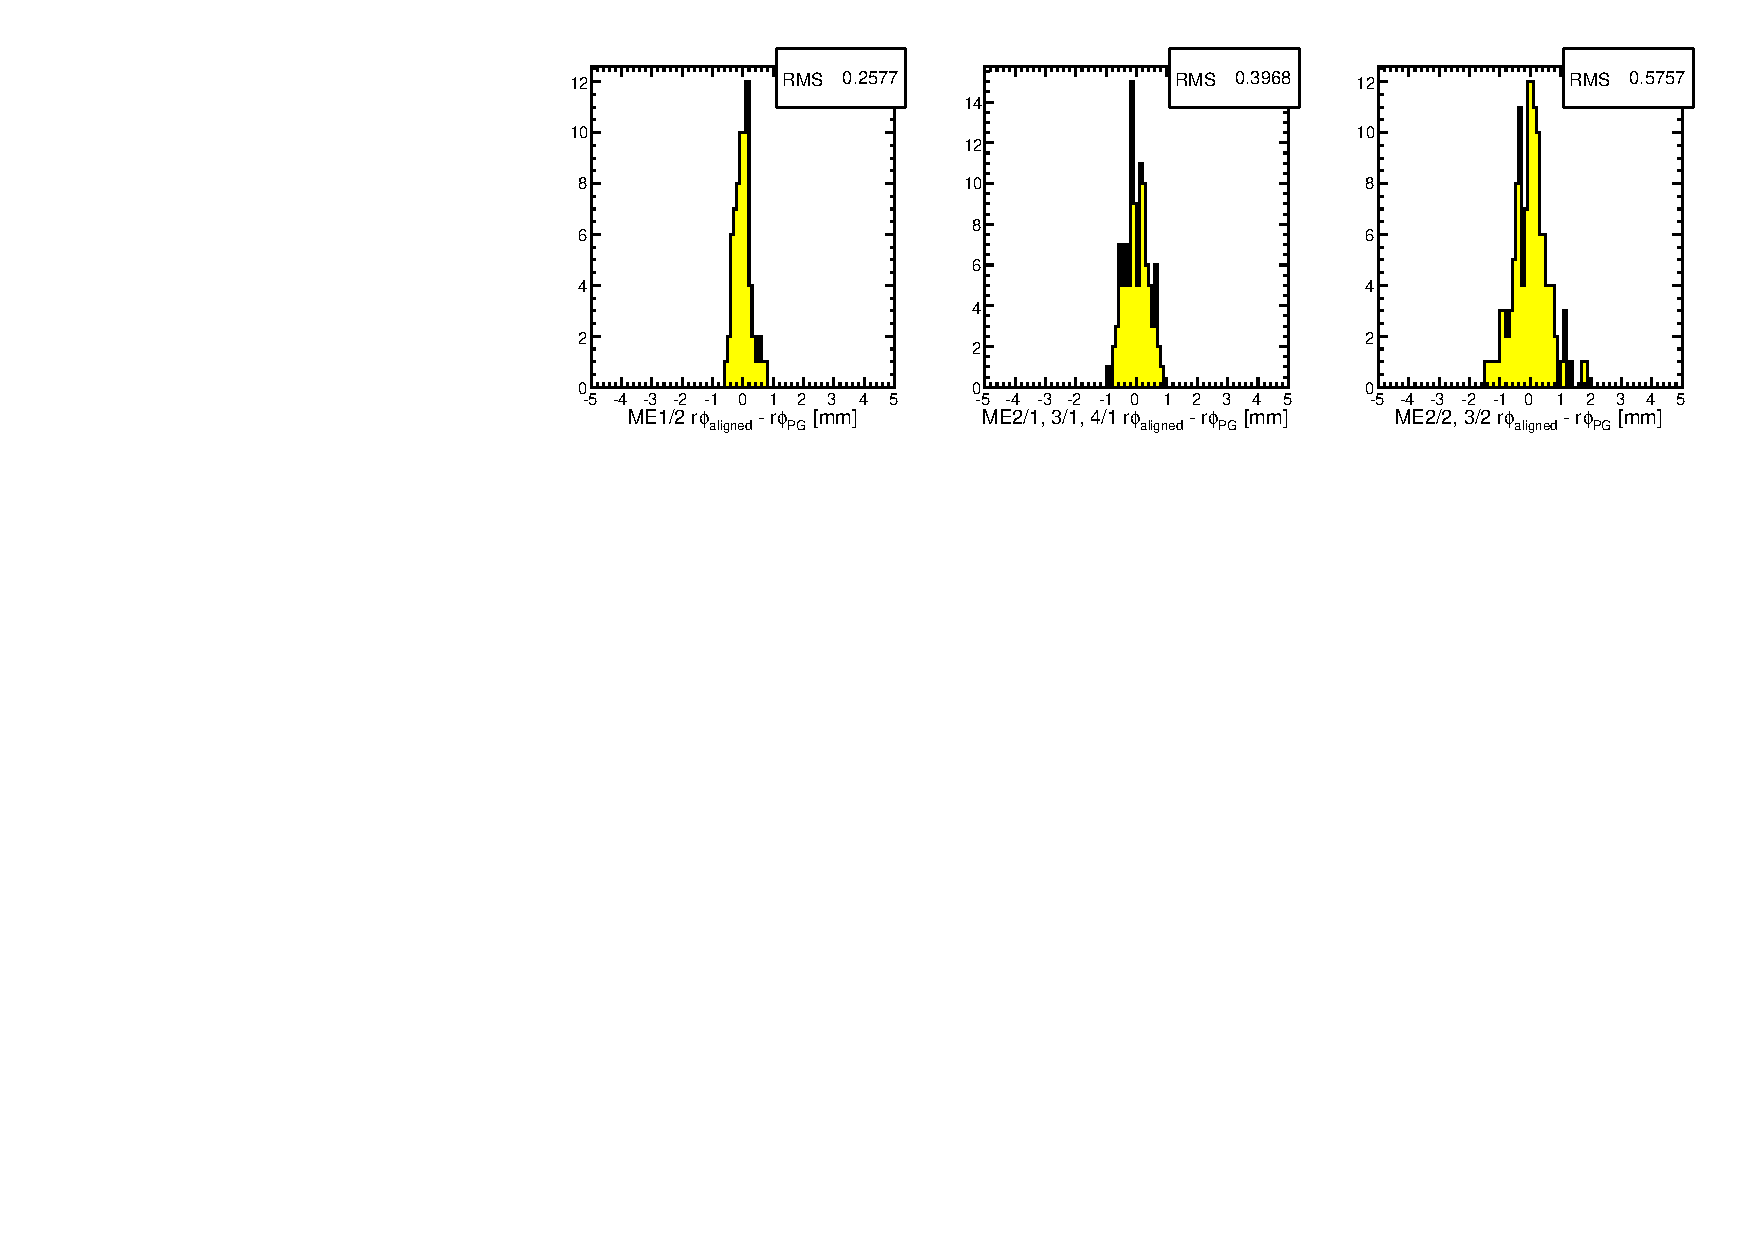
\includegraphics[width=\linewidth]{aligned_minus_pg.pdf}

\caption{Chamber positions after internal-ring alignment compared
  with photogrammetry, split by ring.  (ME1/1 chambers were not
  measured by the photogrammetry.) \label{fig:aligned_minus_pg}}
\end{figure}

\section{Whole-ring placement using collisions muons}

To complete the endcap alignment, the internally aligned rings must be
aligned relative to one another and the tracker.  Tracks from the
tracker were propagated to the muon chambers and whole-ring
corrections were derived from the pattern of $r\phi$ residuals as a
function of global $\phi$.  A constant offset in the residuals is
interpreted as a rotation of the ring in $\phi_z$, while terms
proportional to $\cos\phi$ and $\sin\phi$ are interpreted as
displacements in global $x$ and $y$, respectively.

Figure~\ref{fig:one_and_only_mapplot} provides an example of an
alignment fit for one ring (ME$-$2/1).  The residuals distribution
shows no apparent chamber-level misalignments in the form of
discontinuities at the chamber boundaries.  Residuals were fitted to
truncated Gaussians to determine their peak positions in a way that is
insensitive to non-Gaussian tails.  Residuals from muons and antimuons
were fitted separately and then averaged to reduced sensitivity to any
errors in the magnetic field map, which would affect propagated tracks
of opposite charges in opposite directions with equal magnitude.
Finally, these points were fitted to
\begin{equation}
f(\phi) = c_0 + c_1 \cos\phi + c_2 \sin\phi
\end{equation}
and $c_0$, $c_1$, $c_2$ were used to align the rings.  A second
alignment pass was performed to verify the correction, and was found
to be consistent.

\begin{figure}
\begin{center}
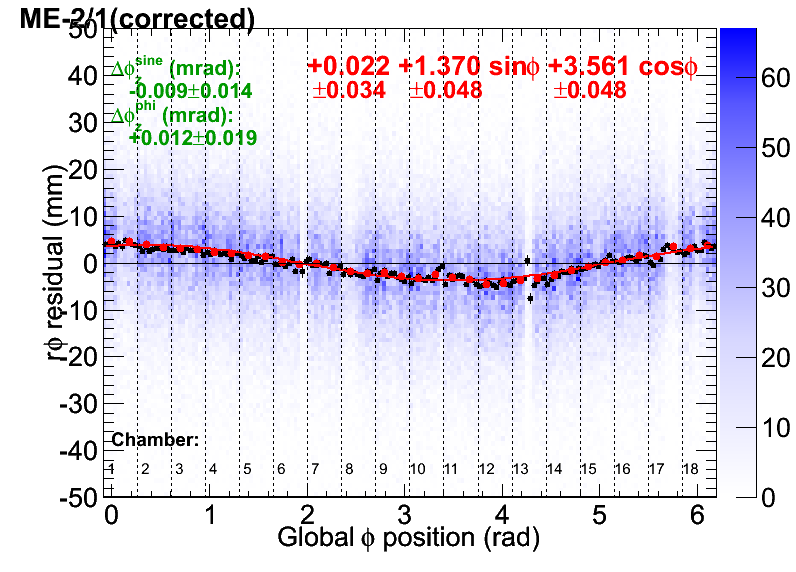
\includegraphics[width=0.5\linewidth]{one_and_only_mapplot.png}
\end{center}

\caption{Residuals plot used to align a ring: the color scale is the
  residuals distribution versus $\phi$, black points are a profile
  derived from truncated-Gaussian peak fits in each $\phi$ bin, and
  red points are the average of peak-fits to muons and antimuons
  separately.  The fitted curve is interpreted as three alignment
  degrees of freedom.  Vertical dashed lines indicate the boundaries
  between chambers. \label{fig:one_and_only_mapplot}}
\end{figure}

To cross-check the alignment using a qualitatively different method,
beam-halo tracks crossing an entire endcap (three or four stations,
depending on distance from the beamline) were used to calculate
residuals in one station relative to segments in another.
Figure~\ref{fig:BHCrossCheck_mep41} shows an example, in which
ME$+$3/1 segments were propagated linearly (no corrections for
material or magnetic field) to ME$+$4/1.  Residuals were fitted with
truncated Gaussians in $\phi$ slices, separately for muons and
antimuons to correct for the magnetic field.

\begin{figure}
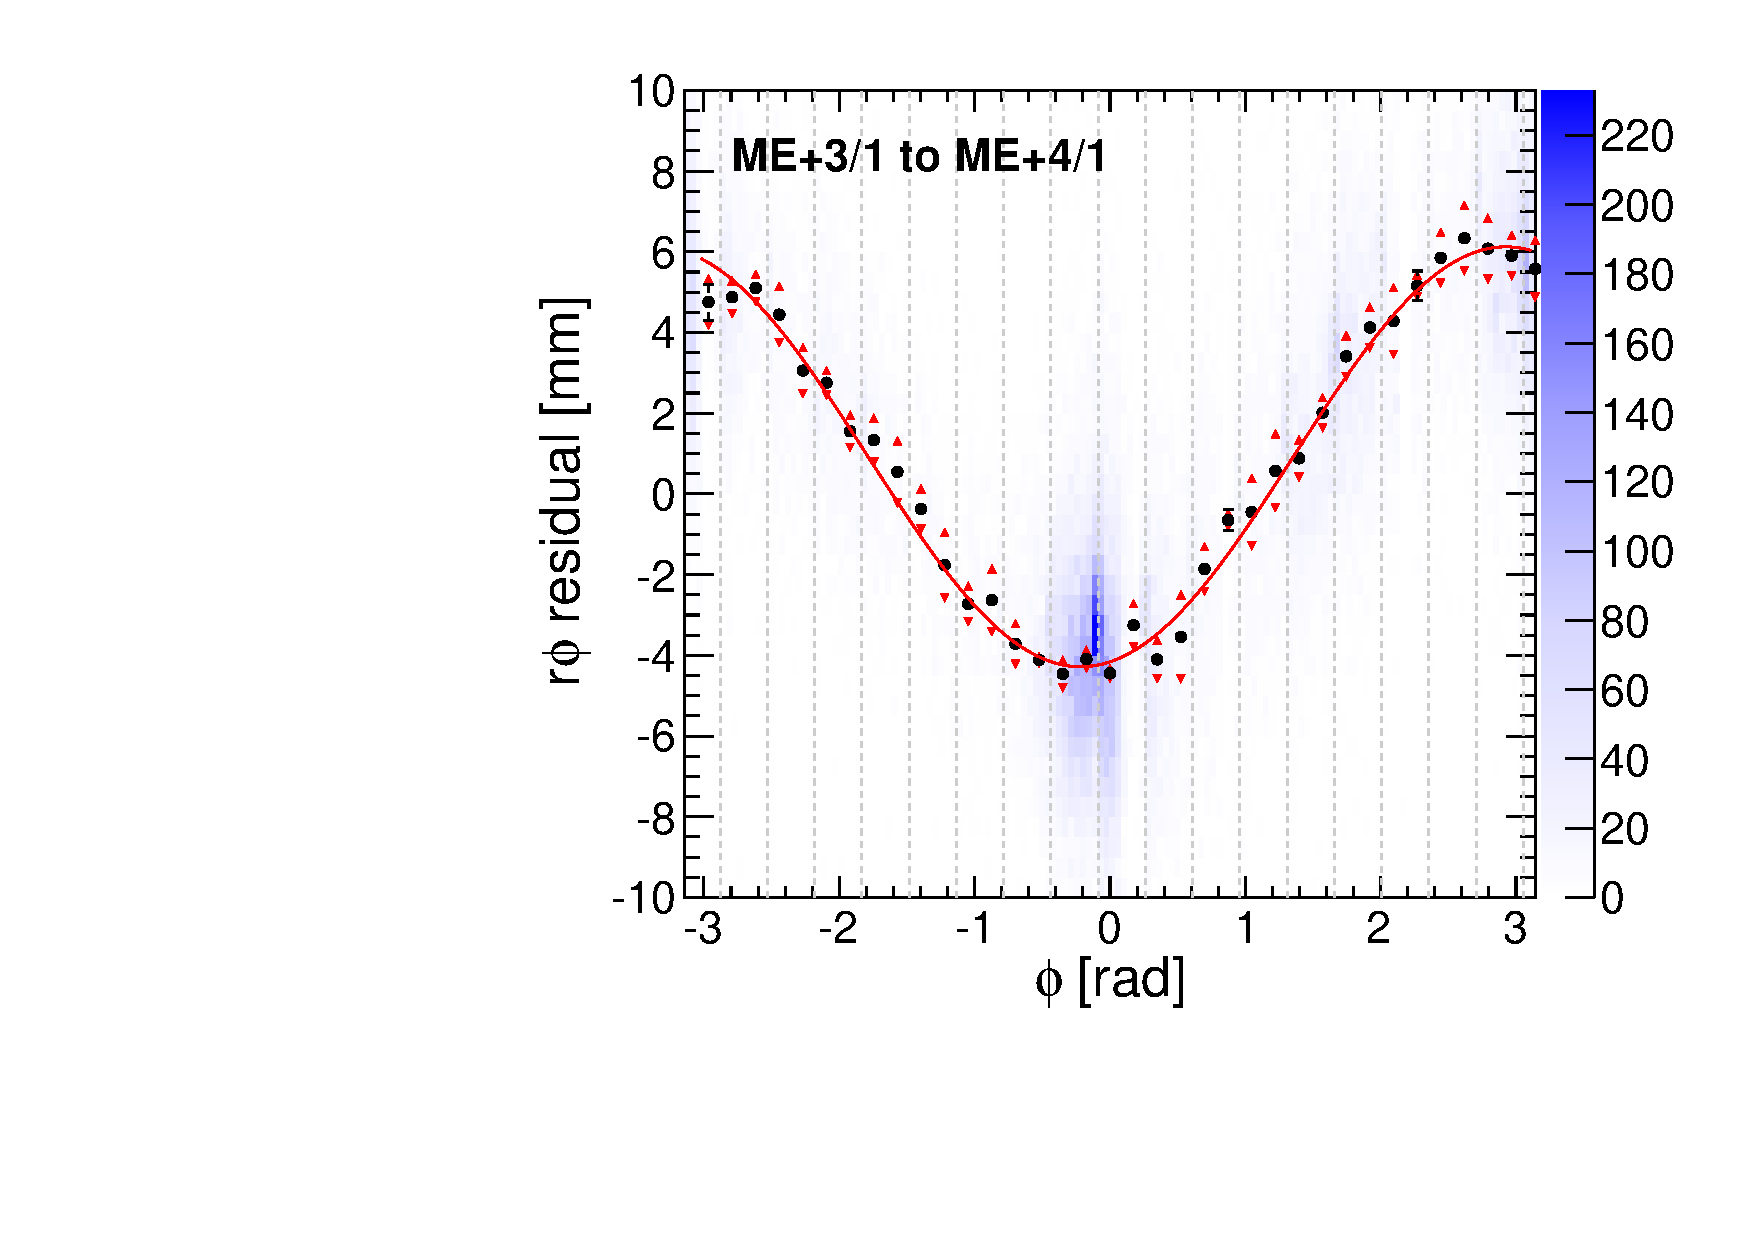
\includegraphics[width=0.45\linewidth]{BHCrossCheck_mep41_before.pdf} \hfill
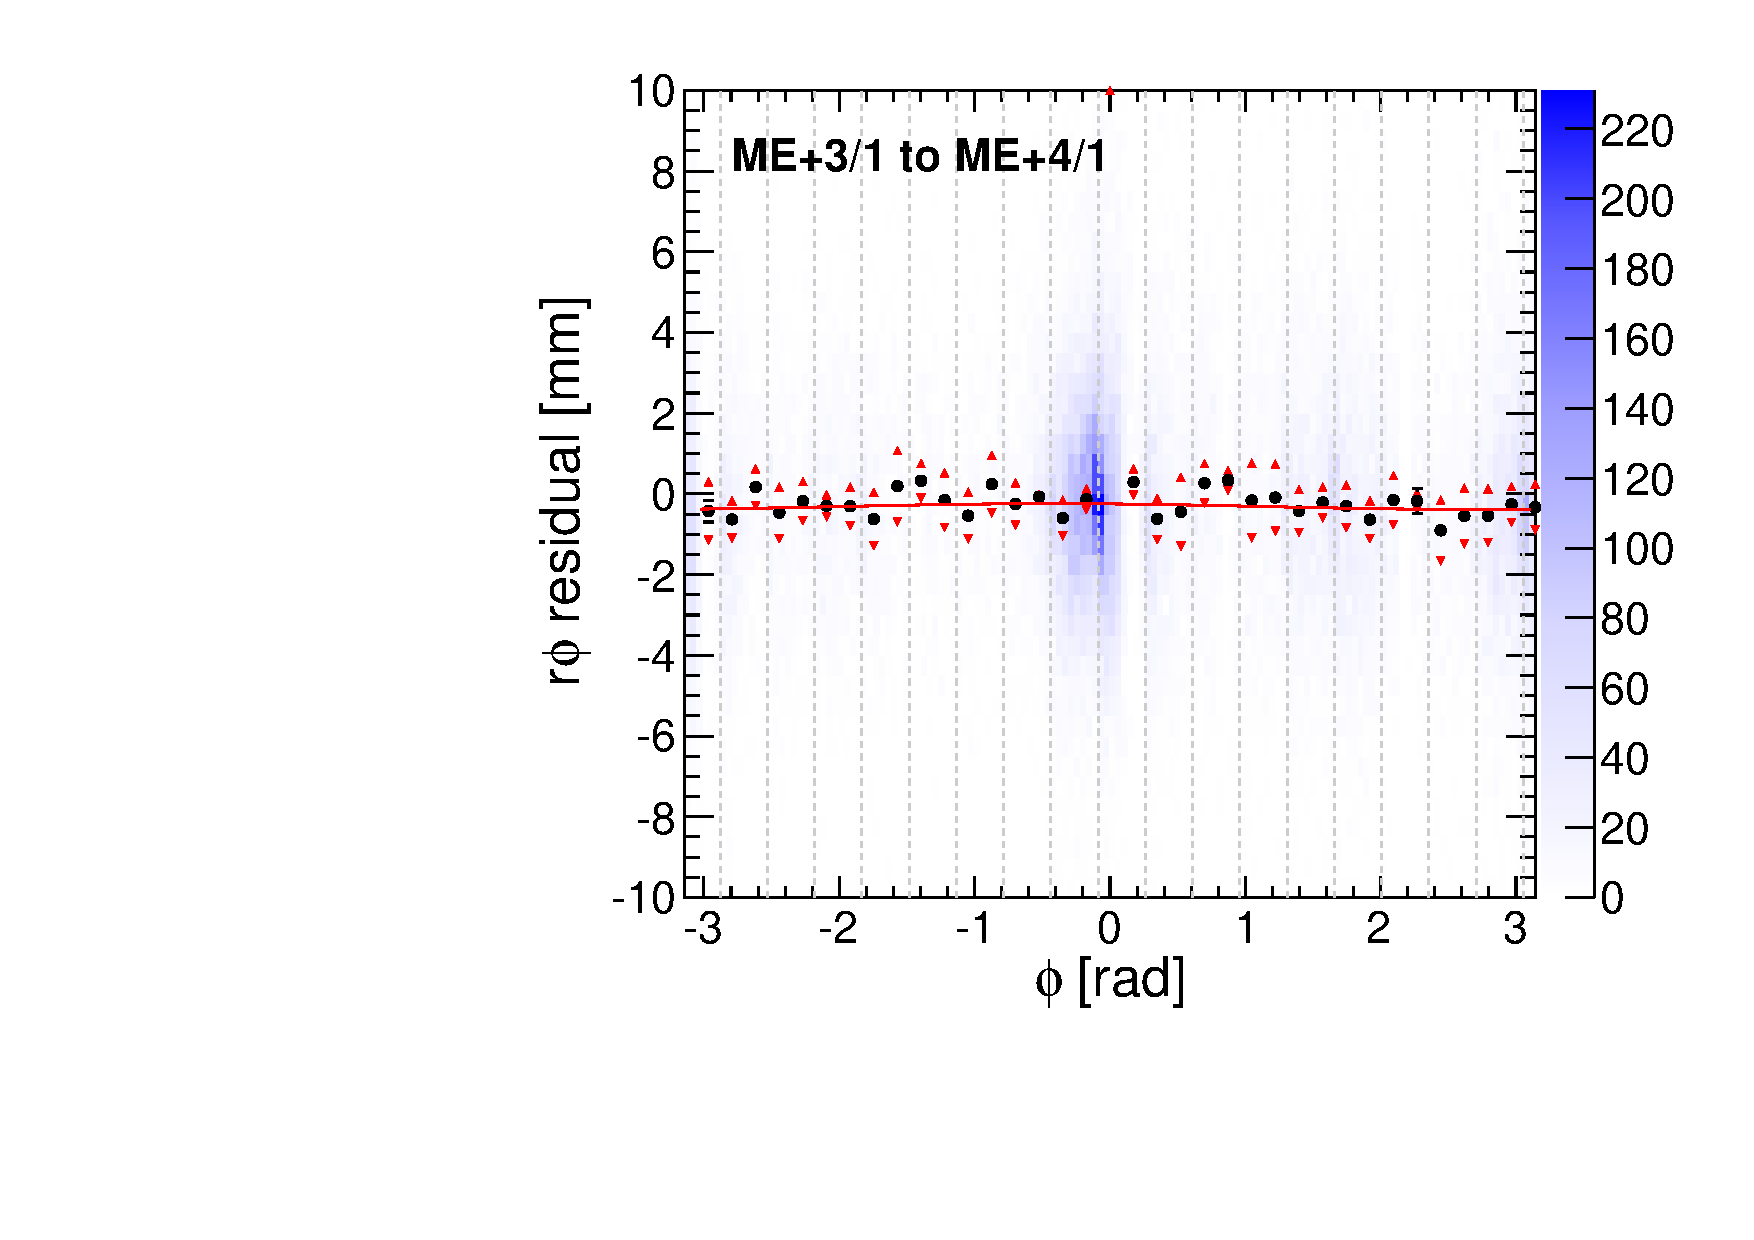
\includegraphics[width=0.45\linewidth]{BHCrossCheck_mep41_after.pdf}

\caption{Residuals from beam-halo tracks used to cross-check the
  alignment performed with collisions.  The symbols in these plots
  have the same meaning as Fig.~\ref{fig:one_and_only_mapplot}, though
  residuals were calculated differently (see text).  Left: before
  alignment.  Right: after alignment using collisions (not
  beam-halo).  \label{fig:BHCrossCheck_mep41}}
\end{figure}

ME4/1 is the farthest station from the CMS tracker, and therefore if
the alignment using tracks from the tracker is compromised by errors
in track propagation, ME4/1 would experience the largest errors.  On
the other hand, the magnetic field is weakest in ME4/1, so the
beam-halo method would have the smallest errors from linear track
propagation and therefore be the most reliable in this station.  As
can be seen in Fig.~\ref{fig:BHCrossCheck_mep41}, the beam-halo
cross-check agrees with the tracker-track alignment at the level of
0.5~mm in ME$+$4/1 (and 0.3~mm in ME$-$4/1, not shown), establishing
an upper bound on ring position errors of 0.5~mm throughout the
endcap.

\section{Conclusions}

The endcap muon system was aligned using several complementary
techniques.  These alignments provide a precise geometry for CMS
tracking and a baseline for comparison with future alignment
techniques.

\end{document}
